\documentclass[aspectratio=169,12pt]{beamer}

% --- Pacotes ---
\usepackage[utf8]{inputenc}
\usepackage[T1]{fontenc}
\usepackage[brazilian]{babel}
\usepackage{graphicx}
\usepackage{xcolor}
\usepackage{tcolorbox}
\usepackage{fontawesome5}

% --- Cores da marca PlanEvidences ---
\definecolor{peGreen}{HTML}{1E9E22}
\definecolor{peGreenDark}{HTML}{167018}
\definecolor{peBg}{HTML}{0F1419}
\definecolor{peSurface}{HTML}{1A1F26}
\definecolor{peText}{HTML}{E5E7EB}
\definecolor{peMuted}{HTML}{9CA3AF}
\definecolor{peAccent}{HTML}{1E9E22}

% --- Tema customizado ---
\usetheme{default}
\setbeamercolor{background canvas}{bg=white}
\setbeamercolor{normal text}{fg=black,bg=white}
\setbeamercolor{frametitle}{fg=peGreen,bg=white}
\setbeamercolor{title}{fg=peGreen}
\setbeamercolor{author}{fg=peMuted}
\setbeamercolor{date}{fg=peMuted}
\setbeamercolor{itemize item}{fg=peGreen}
\setbeamercolor{itemize subitem}{fg=peGreen}
\setbeamercolor{enumerate item}{fg=peGreen}
\setbeamercolor{block title}{fg=white,bg=peGreen}
\setbeamercolor{block body}{fg=black,bg=peGreen!10}
\setbeamertemplate{navigation symbols}{}
\setbeamertemplate{frametitle}{%
  \vspace{0.6em}%
  \hspace{0.5em}\textbf{\Large\insertframetitle}%
  \par\hspace{0.5em}{\color{peGreen}\rule{0.5\linewidth}{2pt}}%
  \vspace{0.3em}%
}
\setbeamertemplate{footline}{%
  \hfill\textcolor{peMuted}{\tiny PlanEvidences QA Suite \quad\textbullet\quad Manual de Uso \quad\textbullet\quad \insertframenumber/\inserttotalframenumber}\hspace{1em}\vspace{0.4em}%
}
\setbeamertemplate{itemize item}{\textcolor{peGreen}{\faChevronRight}}
\setbeamertemplate{itemize subitem}{\textcolor{peGreen}{\textbullet}}

% --- Caixa de destaque "Dica" ---
\newtcolorbox{dica}[1][]{
  colback=peGreen!8,
  colframe=peGreen,
  arc=4pt,
  boxrule=1pt,
  left=8pt,right=8pt,top=4pt,bottom=4pt,
  title={\faLightbulb~Dica},
  fonttitle=\bfseries\color{white},
  colbacktitle=peGreen,
  #1
}

\newtcolorbox{atencao}[1][]{
  colback=orange!10,
  colframe=orange!80!black,
  arc=4pt,
  boxrule=1pt,
  left=8pt,right=8pt,top=4pt,bottom=4pt,
  title={\faExclamationTriangle~Atenção},
  fonttitle=\bfseries\color{white},
  colbacktitle=orange!80!black,
  #1
}

% --- Metadata ---
\title{\Huge\textbf{PlanEvidences}\\[0.3em]\large QA Suite}
\subtitle{\large Manual de Uso para QAs}
\author{Equipe de Qualidade Sudoeste}
\date{\today}

\begin{document}

% =====================================================
% CAPA
% =====================================================
\begin{frame}[plain]
  \begin{center}
    \vspace{1.5cm}
    {\color{peGreen}\rule{0.6\linewidth}{4pt}}\\[1.2em]
    {\Huge\textbf{\color{peGreen}PlanEvidences}}\\[0.4em]
    {\Large\color{peMuted}QA Suite — Manual de Uso}\\[2em]
    {\large Gerador de Casos de Teste\\ + Editor de Evidências}\\[3em]
    {\small\color{peMuted}Equipe de Qualidade Sudoeste \quad\textbullet\quad \today}\\
    \vspace{0.5cm}
    {\color{peGreen}\rule{0.6\linewidth}{2pt}}
  \end{center}
\end{frame}

% =====================================================
% O QUE É
% =====================================================
\begin{frame}{O que é o PlanEvidences?}
  \begin{center}
    \textbf{Acesso (intranet):}\quad\texttt{\color{peGreen}\large http://136.248.115.65:4500}
  \end{center}
  \vspace{0.5em}
  \begin{columns}[T]
    \begin{column}{0.48\textwidth}
      \begin{block}{\faRocket~Gerador de Casos}
        Cole uma HU (ou importe PDF/DOCX/JSON) e a \textbf{IA gera os casos em BDD}.
      \end{block}
      \vspace{0.3em}
      \small
      \begin{itemize}
        \item Heurísticas aplicáveis automáticas
        \item Análise de cobertura e riscos
        \item Status passou/falhou + histórico
      \end{itemize}
    \end{column}
    \begin{column}{0.48\textwidth}
      \begin{block}{\faClipboard~Editor de Evidências}
        Anexa \textbf{prints aos cenários} e \textbf{compila o PDF final} em LaTeX.
      \end{block}
      \vspace{0.3em}
      \small
      \begin{itemize}
        \item Auto-save no Supabase
        \item URL pra colaboração em tempo real
        \item Múltiplos QAs editando junto
      \end{itemize}
    \end{column}
  \end{columns}
\end{frame}

% =====================================================
% GERADOR — TELA INICIAL
% =====================================================
\begin{frame}{Gerador de Casos — Tela Inicial}
  \begin{columns}[T]
    \begin{column}{0.6\textwidth}
      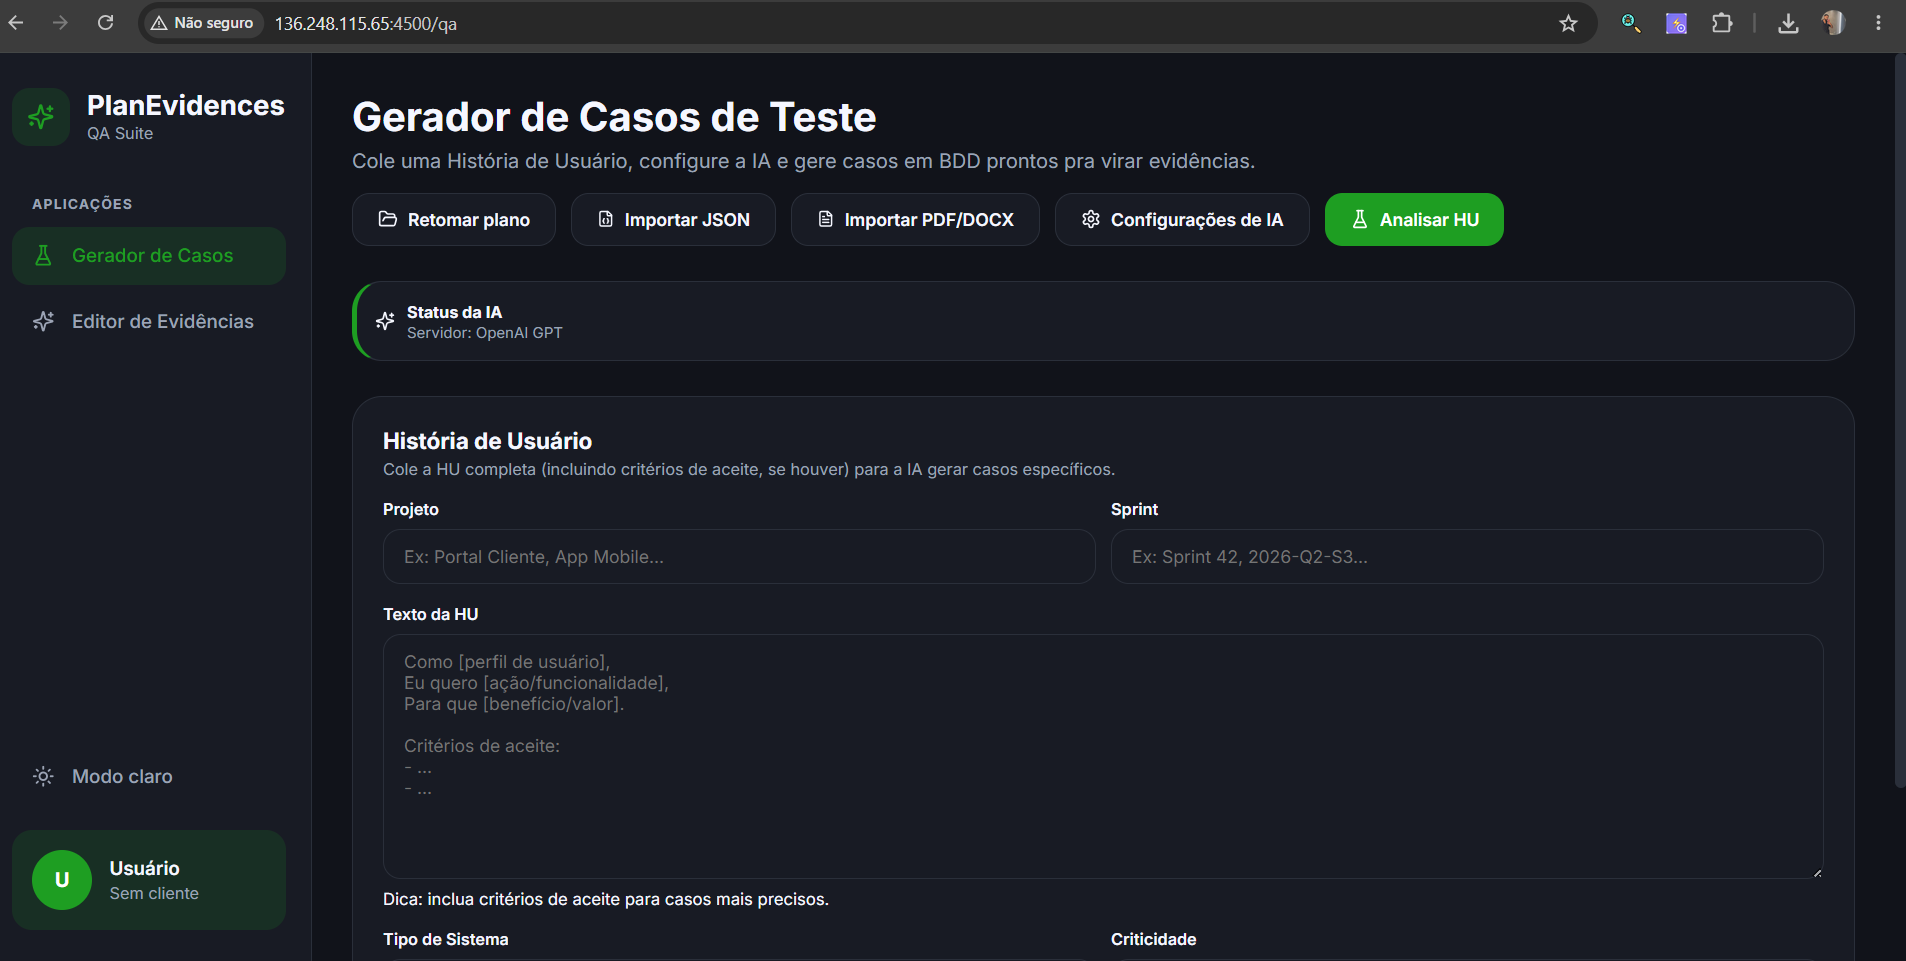
\includegraphics[width=\linewidth]{images/01-qa-home.png}
    \end{column}
    \begin{column}{0.37\textwidth}
      \footnotesize
      \textbf{Sidebar:} Gerador de Casos (\texttt{/qa}) e Editor de Evidências (\texttt{/evidences}).
      \vspace{0.5em}

      \textbf{Header (botões):}
      \begin{itemize}
        \item Retomar plano
        \item Importar JSON / PDF / DOCX
        \item Configurações de IA
        \item \textbf{Analisar HU} (verde)
      \end{itemize}
      \vspace{0.5em}

      \textbf{Status da IA} — mostra se está usando key do servidor ou do navegador.
    \end{column}
  \end{columns}
\end{frame}

% =====================================================
% CONFIGURAR IA
% =====================================================
\begin{frame}{Configurando a IA (1ª vez)}
  \small
  \textbf{Quando:} se o status mostrar \textit{``IA não configurada''} (badge vermelho).
  \vspace{0.3em}
  \begin{enumerate}
    \item Clique \textbf{Configurações de IA}
    \item Escolha o provedor: \textbf{Gemini} (grátis), \textbf{Anthropic} (pago) ou \textbf{OpenAI}
    \item Escolha o modelo (default já é o recomendado)
    \item Cole a \textbf{API Key} → \textbf{Testar conexão} → \textbf{Salvar}
  \end{enumerate}
  \vspace{0.3em}
  \begin{dica}
    A chave fica salva \textbf{só no seu navegador}. Se o servidor já tiver uma key, ela é usada por padrão.
  \end{dica}
\end{frame}

% =====================================================
% PREENCHER HU
% =====================================================
\begin{frame}{Preencher a HU e analisar}
  \begin{columns}[T]
    \begin{column}{0.6\textwidth}
      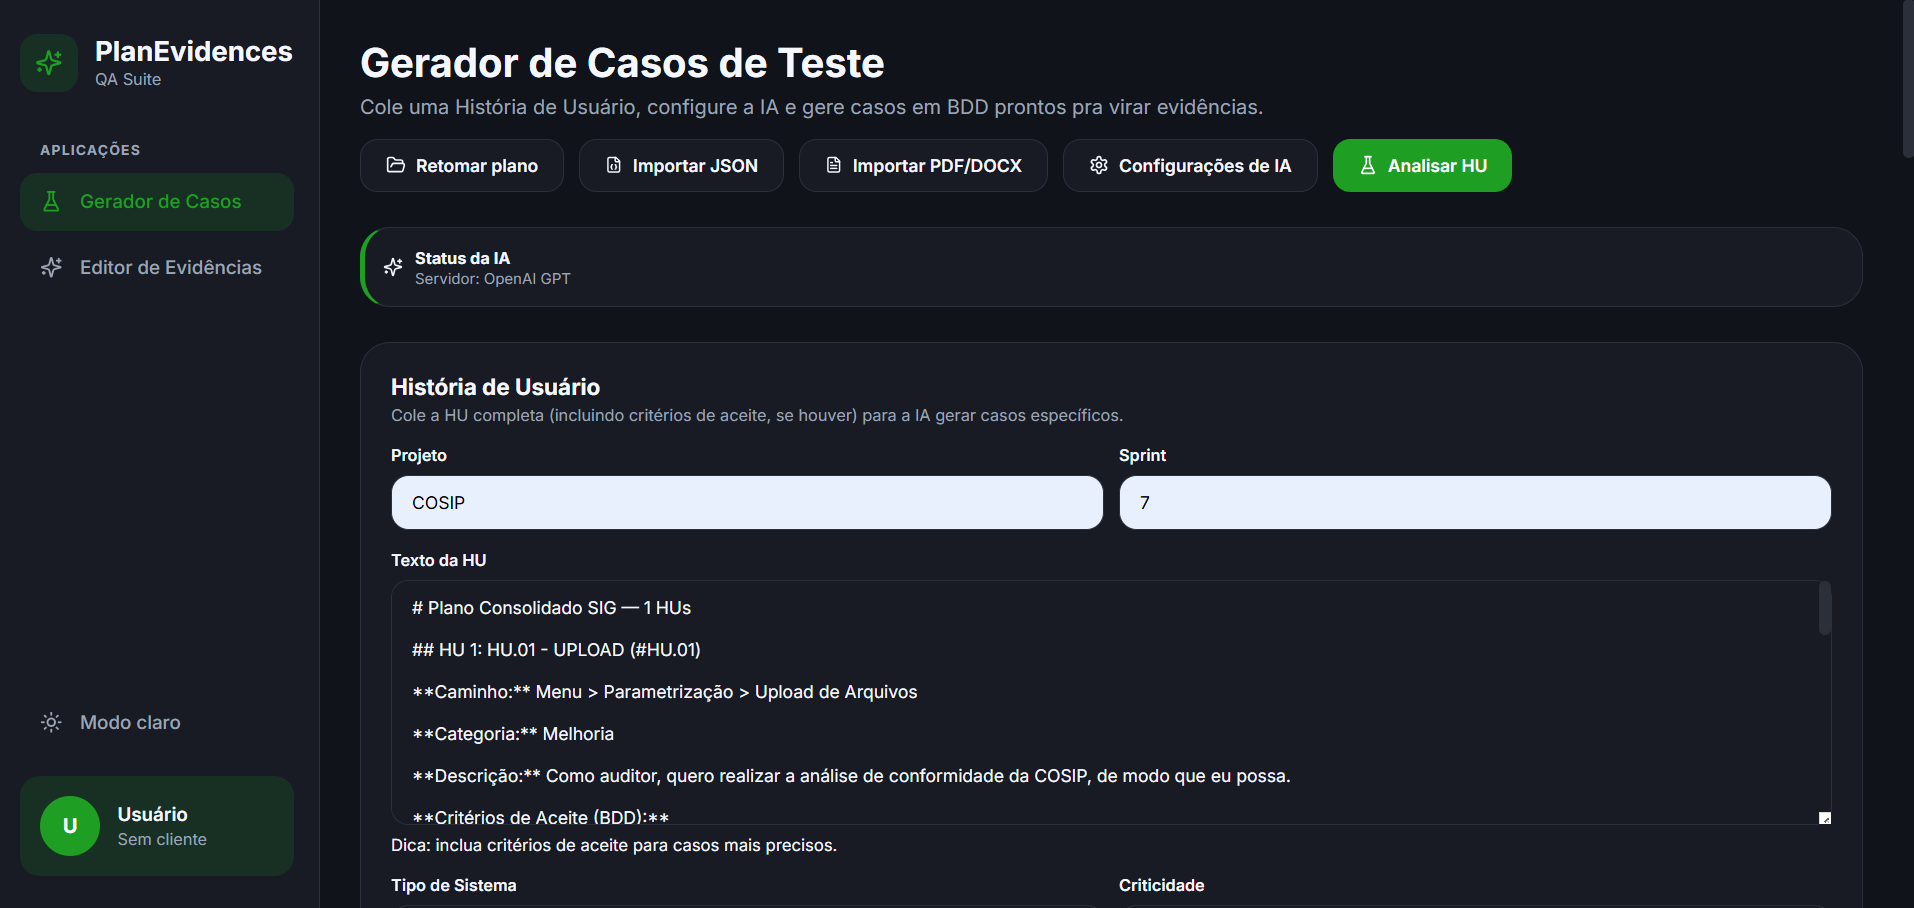
\includegraphics[width=\linewidth]{images/03-qa-hu-preenchida.png}
    \end{column}
    \begin{column}{0.37\textwidth}
      \footnotesize
      \textbf{Duas formas de entrar com a HU:}
      \begin{enumerate}
        \item \textbf{Colar texto} no campo \textit{Texto da HU}
        \item \textbf{Importar PDF/DOCX/JSON} — botões no header populam automaticamente
      \end{enumerate}
      \vspace{0.4em}
      \textbf{Também preencher:}
      \begin{itemize}
        \item Projeto e Sprint
        \item Tipo (Web/Mobile/API/IA)
        \item Criticidade
      \end{itemize}
      \vspace{0.4em}
      Clique \textbf{Analisar HU} — IA roda em \textbf{20-60s}.
    \end{column}
  \end{columns}
\end{frame}

% =====================================================
% TAB CASOS DE TESTE
% =====================================================
\begin{frame}{Resultado: Tab Casos de Teste}
  \begin{columns}[T]
    \begin{column}{0.65\textwidth}
      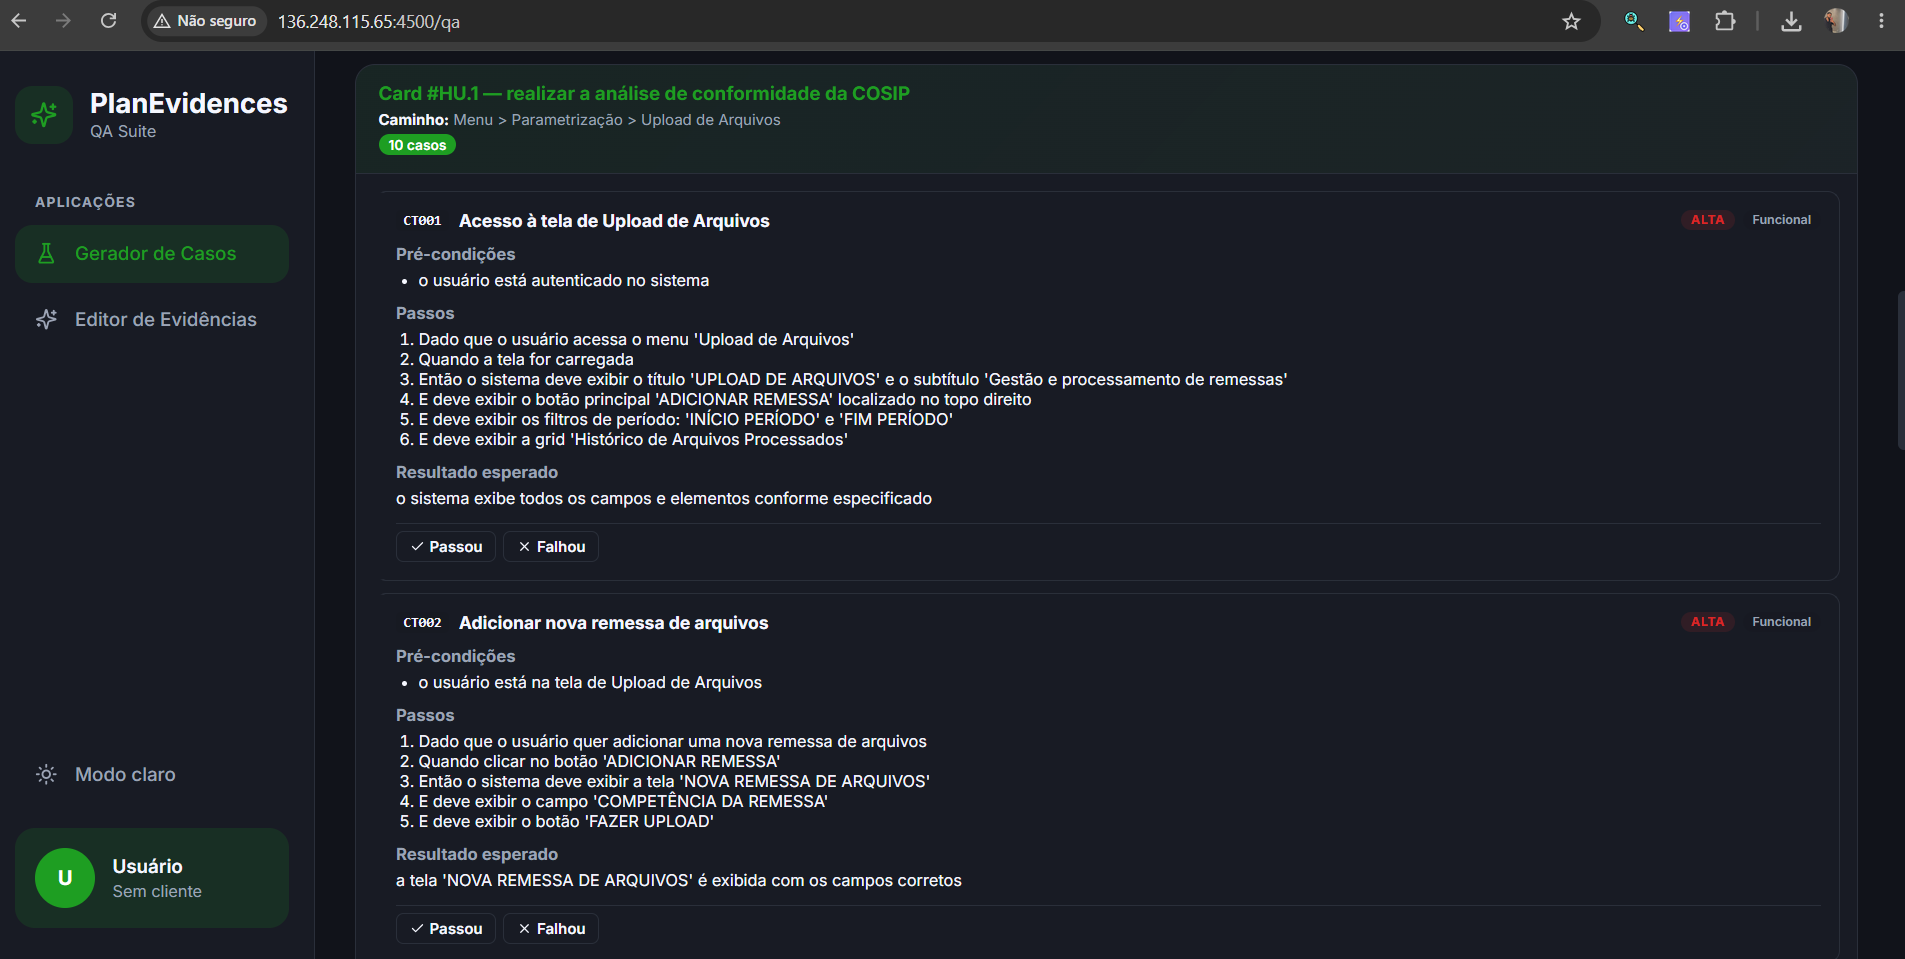
\includegraphics[width=\linewidth]{images/04-casos-teste.png}
    \end{column}
    \begin{column}{0.32\textwidth}
      \footnotesize
      \textbf{Cada caso traz:}
      \begin{itemize}
        \item Código (CT-001…)
        \item Título curto
        \item Pré-condições \textit{(Dado)}
        \item Passos \textit{(Quando)}
        \item Resultado \textit{(Então)}
        \item Prioridade + tipo
      \end{itemize}
      \vspace{0.5em}
      Após salvar no Supabase, surgem os botões \textbf{Passou} / \textbf{Falhou}.
    \end{column}
  \end{columns}
\end{frame}

% =====================================================
% TAB COBERTURA
% =====================================================
\begin{frame}{Tab Cobertura e Riscos}
  \begin{columns}[T]
    \begin{column}{0.7\textwidth}
      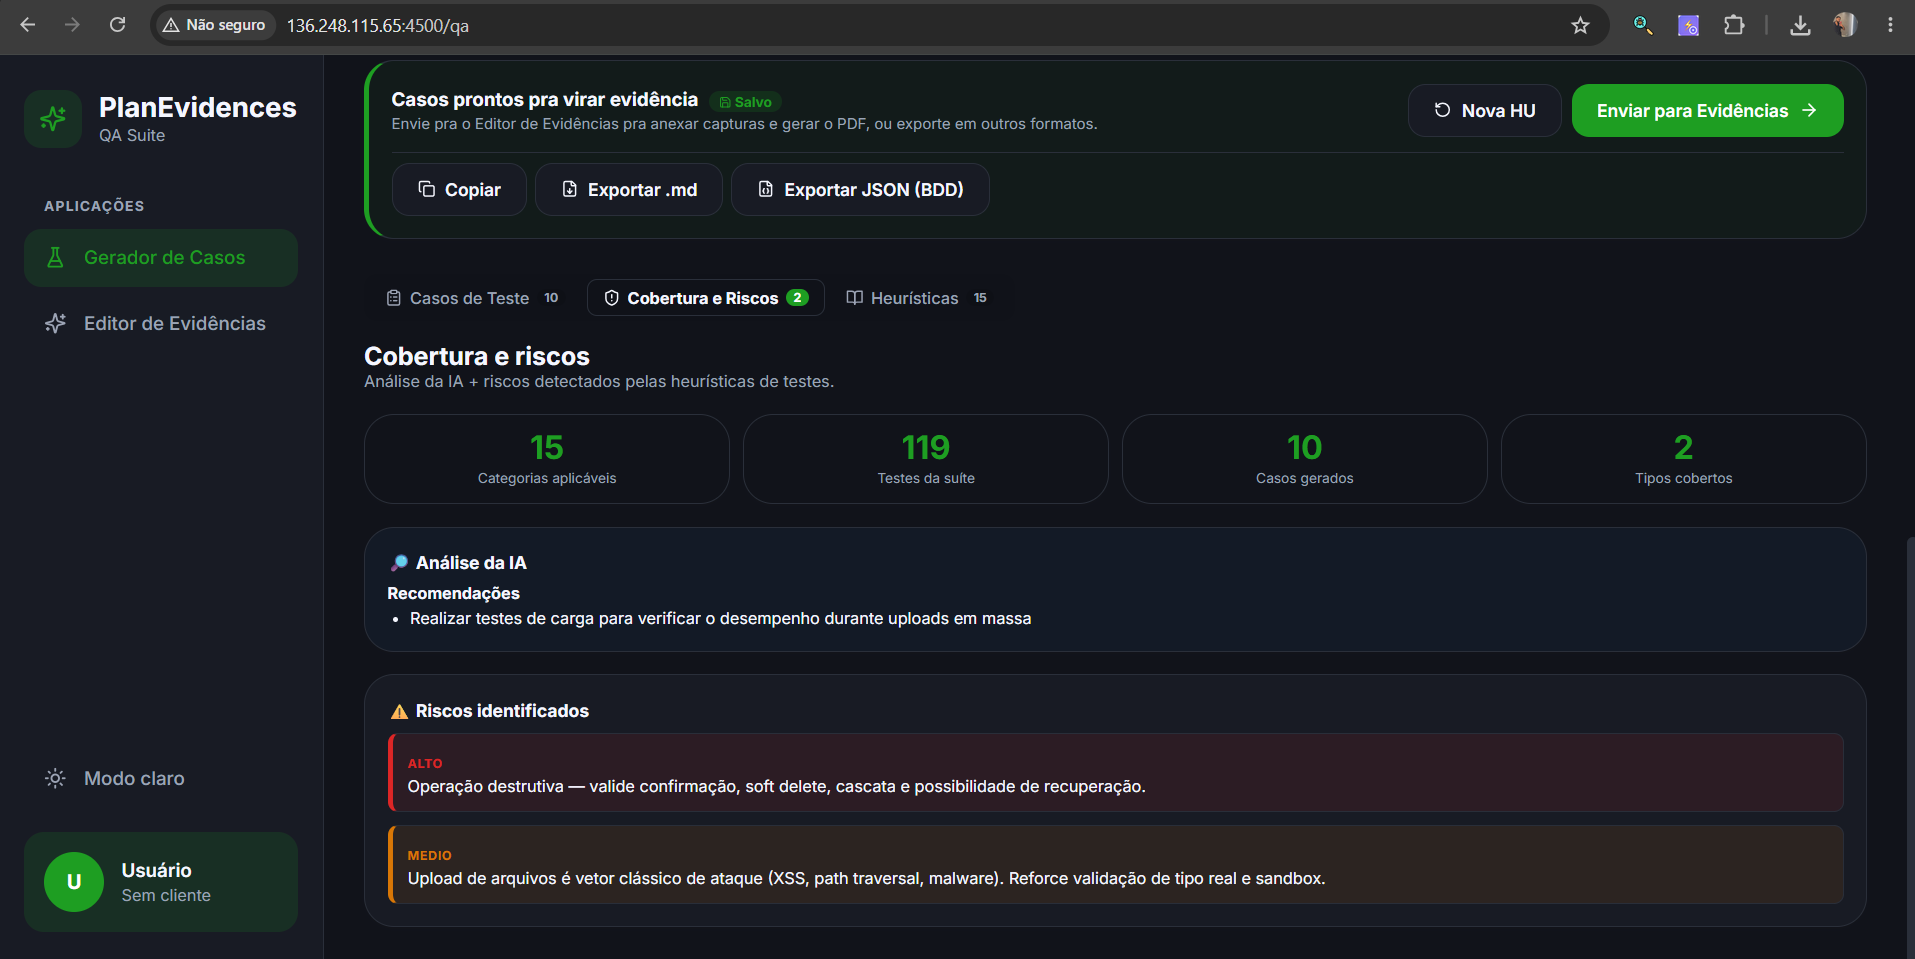
\includegraphics[width=\linewidth]{images/05-cobertura-riscos.png}
    \end{column}
    \begin{column}{0.27\textwidth}
      \footnotesize
      \textbf{Métricas (topo)}
      \vspace{0.3em}

      \textbf{Análise da IA:}
      \begin{itemize}
        \item Ambiguidades
        \item Perguntas pro PO
        \item Recomendações
      \end{itemize}
      \vspace{0.3em}

      \textbf{Riscos} (badges coloridos por gravidade)
    \end{column}
  \end{columns}
\end{frame}

% =====================================================
% TAB HEURÍSTICAS
% =====================================================
\begin{frame}{Tab Heurísticas Aplicáveis}
  \begin{columns}[T]
    \begin{column}{0.65\textwidth}
      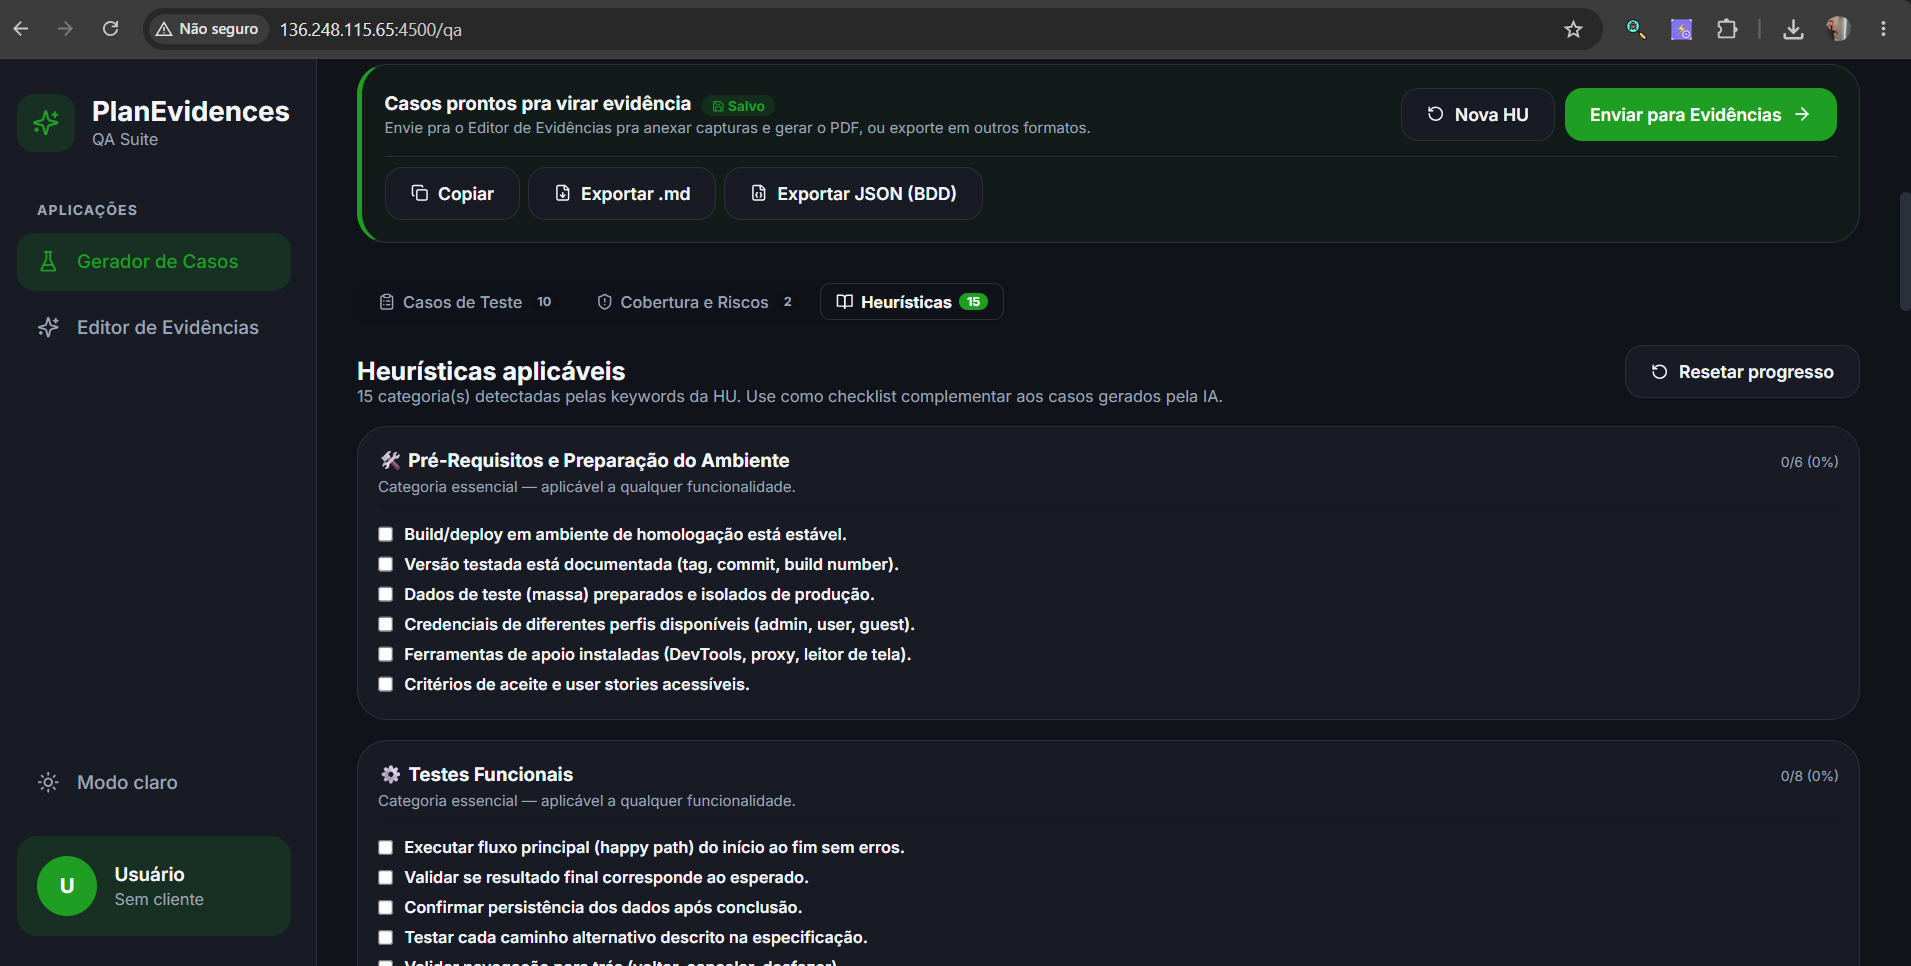
\includegraphics[width=\linewidth]{images/06-heuristicas.png}
    \end{column}
    \begin{column}{0.32\textwidth}
      \footnotesize
      \textbf{20 categorias} — filtradas pelas keywords da HU.

      \vspace{0.4em}
      Funciona como \textbf{checklist complementar}. Cada item tem checkbox; o progresso \textbf{persiste por HU}.

      \vspace{0.4em}
      Cobre: Funcionais, CRUD, Segurança, Acessibilidade, UX, Performance, etc.
    \end{column}
  \end{columns}
\end{frame}

% =====================================================
% RETOMAR PLANO
% =====================================================
\begin{frame}{Retomar um Plano Salvo}
  \begin{columns}[T]
    \begin{column}{0.6\textwidth}
      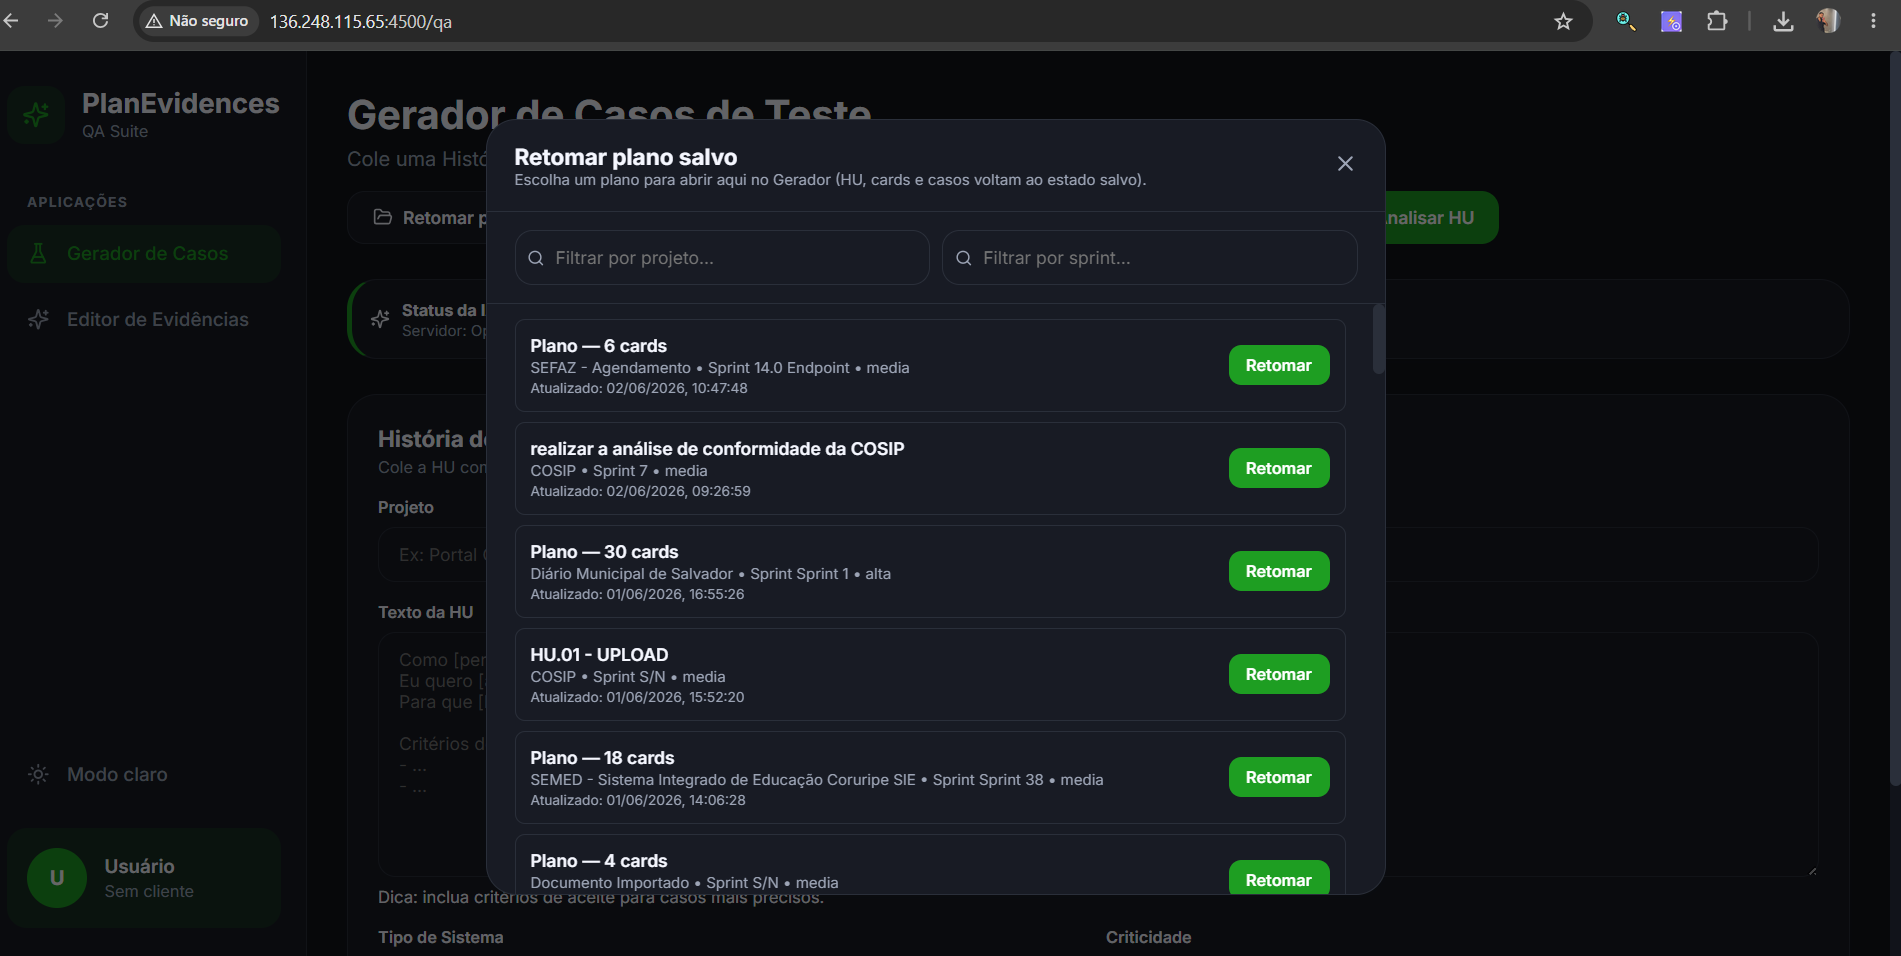
\includegraphics[width=\linewidth]{images/02-retomar-plano.png}
    \end{column}
    \begin{column}{0.37\textwidth}
      \footnotesize
      Cada análise é \textbf{salva automaticamente} no Supabase.

      \vspace{0.4em}
      Pra abrir uma análise antiga:
      \begin{enumerate}
        \item Clique \textbf{Retomar plano}
        \item Filtre por Projeto ou Sprint
        \item Clique \textbf{Retomar}
      \end{enumerate}

      \vspace{0.4em}
      HU, cards, casos e status voltam como estavam.
    \end{column}
  \end{columns}
\end{frame}

% =====================================================
% ENVIAR PRA EVIDÊNCIAS
% =====================================================
\begin{frame}{Enviar para Evidências}
  \small
  Depois que a IA gerar os casos, clique no botão verde \textbf{Enviar para Evidências} (header dos resultados).

  \vspace{0.5em}
  \textbf{O que acontece:}
  \begin{itemize}
    \item Casos viram \textbf{cenários BDD} (Dado/Quando/Então)
    \item Editor abre \textbf{populado automaticamente}
    \item Cards de origem ficam preservados como agrupamento
  \end{itemize}

  \vspace{0.5em}
  \begin{dica}
    Sem ir pra evidências, dá pra exportar via \textbf{Copiar} (Markdown), \textbf{Exportar .md} ou \textbf{Exportar JSON (BDD)} pra ferramentas externas.
  \end{dica}
\end{frame}

% =====================================================
% EDITOR DE EVIDÊNCIAS
% =====================================================
\begin{frame}{Editor de Evidências — Visão Geral}
  \begin{columns}[T]
    \begin{column}{0.65\textwidth}
      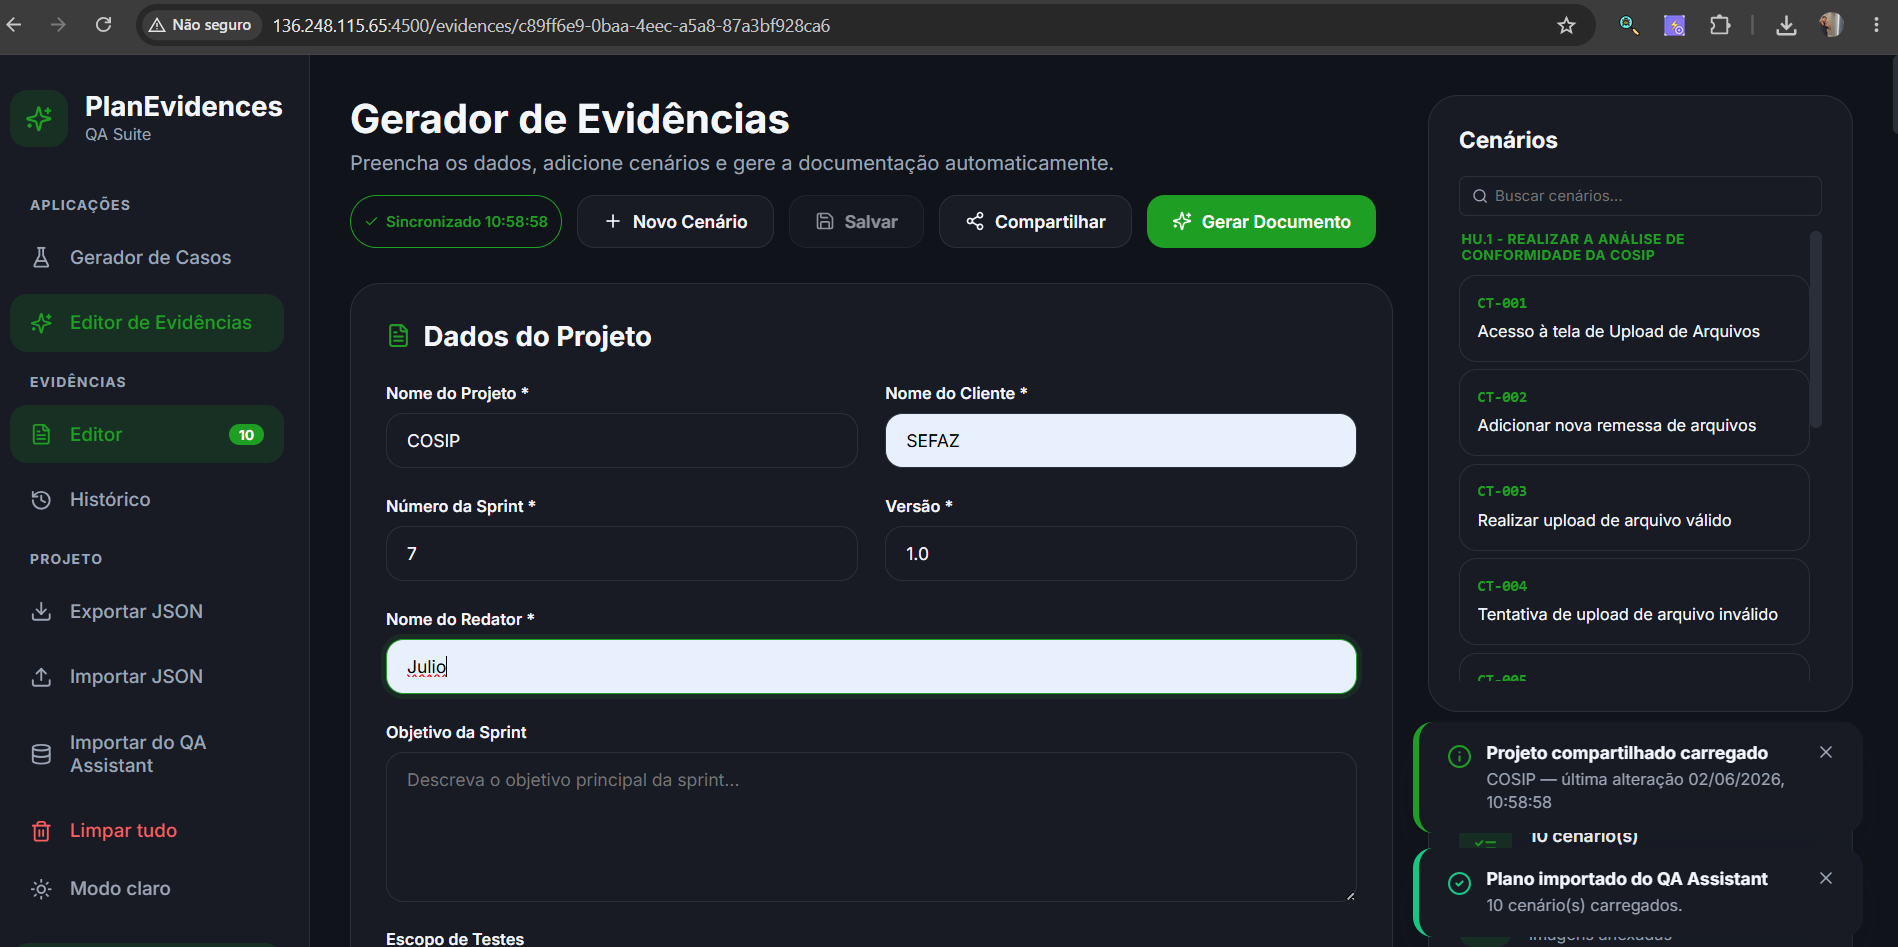
\includegraphics[width=\linewidth]{images/07-editor-evidencias.png}
    \end{column}
    \begin{column}{0.32\textwidth}
      \footnotesize
      \textbf{Dados do Projeto:}
      Cliente, Sprint, Versão, Redator, Objetivo, Escopo.
      \vspace{0.4em}

      \textbf{Painel direito:} lista de cenários (navegação rápida).
      \vspace{0.4em}

      \textbf{Header — botões:}
      \begin{itemize}
        \item Novo Cenário
        \item Salvar
        \item Compartilhar
        \item Gerar Documento
      \end{itemize}
    \end{column}
  \end{columns}
\end{frame}

% =====================================================
% EDITAR CENÁRIO
% =====================================================
\begin{frame}{Editando um Cenário}
  \begin{columns}[T]
    \begin{column}{0.65\textwidth}
      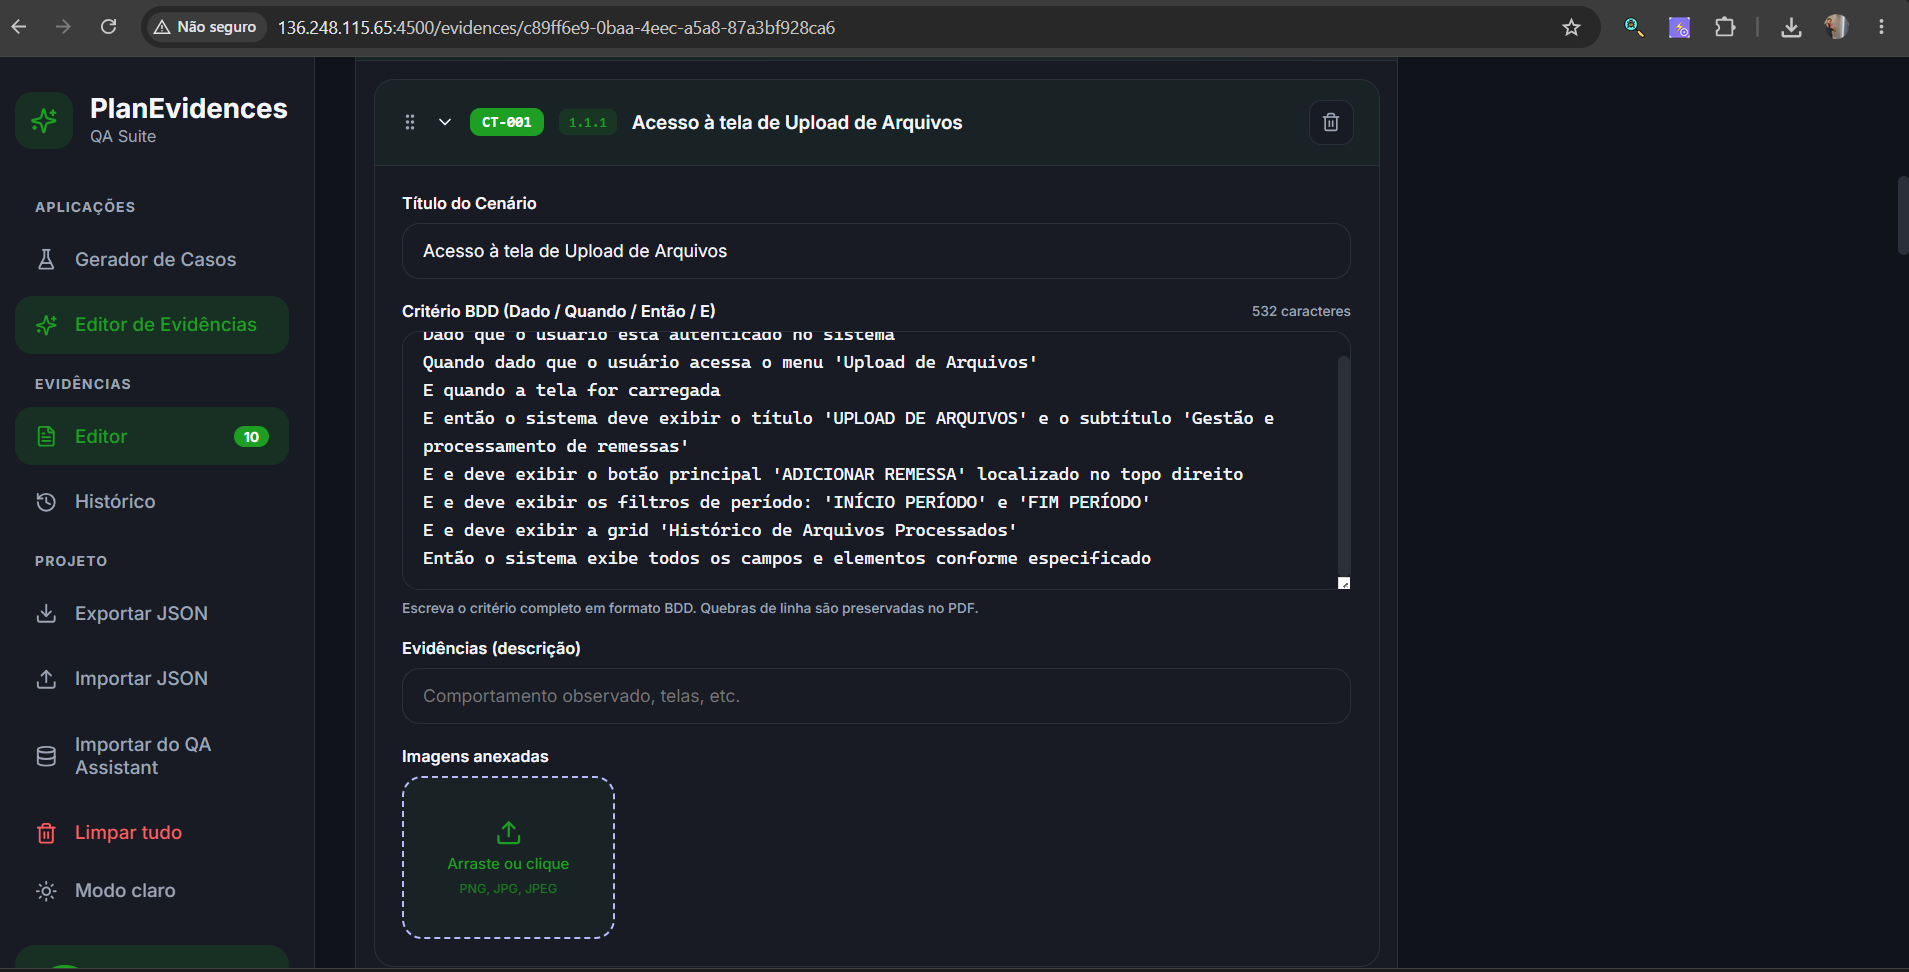
\includegraphics[width=\linewidth]{images/08-editor-cenario.png}
    \end{column}
    \begin{column}{0.32\textwidth}
      \footnotesize
      \textbf{Por cenário:}
      \begin{itemize}
        \item Título
        \item Critério BDD
        \item Evidências (texto)
        \item Imagens (prints)
      \end{itemize}
      \vspace{0.4em}

      \textbf{Anexar prints:}
      arraste/solte na área pontilhada ou clique pra selecionar. Sobe pro Supabase Storage.

      \vspace{0.4em}
      Arraste o cabeçalho do cenário pra \textbf{reordenar}.
    \end{column}
  \end{columns}
\end{frame}

% =====================================================
% COLABORAÇÃO + AUTO-SAVE
% =====================================================
\begin{frame}{Colaboração em Tempo Real}
  \small
  \textbf{Auto-save:} alterações salvam no Supabase em \textbf{3s}. Badge no header:
  \begin{itemize}
    \item \textcolor{peGreen}{\faCheckCircle~\textbf{Sincronizado HH:MM}} — tudo salvo
    \item \textcolor{orange}{\faExclamationCircle~\textbf{Alterações não salvas}} — esperando 3s
    \item \textcolor{peMuted}{\faSync~\textbf{Salvando...}} — gravando agora
  \end{itemize}

  \vspace{0.4em}
  \textbf{Compartilhar:} clique \textbf{Compartilhar} → URL no clipboard → cola no Slack. Outro QA abre e vê o mesmo projeto. Cada save aparece no outro em \textbf{1-2s} (toast \textit{``Atualizado por outro QA''}).

  \vspace{0.3em}
  \begin{atencao}
    Conflito: mesmo cenário, dois QAs ao mesmo tempo → \textbf{último write vence}. Combine quem mexe em quê.
  \end{atencao}
\end{frame}

% =====================================================
% GERAR PDF FINAL
% =====================================================
\begin{frame}{Gerando o PDF Final}
  Quando os cenários estiverem com prints e evidências preenchidos:

  \vspace{0.8em}
  \begin{enumerate}
    \item Confirme \textbf{Cliente}, \textbf{Sprint}, \textbf{Redator} preenchidos
    \item Clique \textbf{Gerar Documento} (verde, header)
    \item Aguarde \textbf{5-15s} (LaTeX compila no servidor)
    \item Aparecem 2 links pra download:
    \begin{itemize}
      \item \textbf{.tex} — código fonte do documento
      \item \textbf{PDF} — versão final pronta pra entregar
    \end{itemize}
  \end{enumerate}

  \vspace{0.8em}
  \begin{dica}
    O documento gerado fica também no \textbf{Histórico} (sidebar). Lá dá pra baixar versões anteriores e reabrir o projeto pra regerar.
  \end{dica}
\end{frame}

% =====================================================
% DICAS FINAIS
% =====================================================
\begin{frame}{Dicas Finais}
  \begin{itemize}
    \item \textbf{HU mais detalhada = casos mais específicos.} Inclua critérios de aceite em bullets.
    \vspace{0.3em}
    \item \textbf{Use as 3 tabs juntas:} a IA gera o plano principal, Heurísticas é seu checklist final, Cobertura mostra o que pode estar faltando.
    \vspace{0.3em}
    \item \textbf{Salve antes de fechar:} mesmo com auto-save, espere ver \textcolor{peGreen}{``Sincronizado''} no badge antes de fechar a aba.
    \vspace{0.3em}
    \item \textbf{Reaproveite:} ``Retomar plano'' carrega análises antigas, evita refazer do zero quando a HU muda pouco.
    \vspace{0.3em}
    \item \textbf{Marque status:} use Passou/Falhou em cada caso conforme executa — o histórico de falhas fica disponível pro próximo ciclo.
    \vspace{0.3em}
    \item \textbf{Compartilhe:} a URL do projeto de evidência permite que 2+ QAs trabalhem juntos no mesmo plano sem atropelar um o outro.
  \end{itemize}
\end{frame}

% =====================================================
% CONTRACAPA
% =====================================================
\begin{frame}[plain]
  \begin{center}
    \vspace{2cm}
    {\color{peGreen}\rule{0.5\linewidth}{3pt}}\\[1.5em]
    {\Large\textbf{Dúvidas, bugs ou sugestões?}}\\[1em]
    {\large Fale com a Equipe de Qualidade Sudoeste}\\[2em]
    {\small\color{peMuted}PlanEvidences QA Suite\\ Manual v1.0 \quad\textbullet\quad \today}\\[2em]
    {\color{peGreen}\rule{0.5\linewidth}{2pt}}
  \end{center}
\end{frame}

\end{document}
